\documentclass[review]{elsarticle}

\usepackage{multirow}
\usepackage{lineno}
\usepackage{xspace}
\usepackage{threeparttable}
\usepackage{subfig}
\modulolinenumbers[5]

%% Journal name here
\journal{FIXME: The Journal Name Goes Here}

%% `Elsevier LaTeX' style
\bibliographystyle{elsarticle-num}
%%%%%%%%%%%%%%%%%%%%%%%

%%%% packages and definitions (optional)
\usepackage{placeins}
\usepackage{booktabs} % nice rules (thick lines) for tables
\usepackage{microtype} % improves typography for PDF
\usepackage{hhline}
\usepackage{amsmath}
\usepackage{subfig}

\usepackage{booktabs}
\usepackage{threeparttable, tablefootnote}

\usepackage{tabularx}

%% Special typesetting for Cyclus
\newcommand{\Cyclus}{\textsc{Cyclus}\xspace}%
\newcommand{\Cycamore}{\textsc{Cycamore}\xspace}%
\graphicspath{{images/}}

% tikz %
\usepackage{tikz}
\usetikzlibrary{positioning, arrows, decorations, shapes}

\usetikzlibrary{shapes.geometric,arrows}
\tikzstyle{process} = [rectangle, rounded corners, minimum width=3cm, minimum height=1cm,text centered, draw=black, fill=blue!30]
\tikzstyle{object} = [ellipse, rounded corners, minimum width=3cm, minimum height=1cm,text centered, draw=black, fill=green!30]
\tikzstyle{arrow} = [thick,->,>=stealth]

% hyperref %
\usepackage[hidelinks]{hyperref}
% after hyperref %
\usepackage{cleveref}
\usepackage{datatool}
\usepackage[acronym,toc]{glossaries}
%\newacronym{<++>}{<++>}{<++>}
\newacronym[longplural={metric tons of heavy metal}]{MTHM}{MTHM}{metric ton of heavy metal}
\newacronym{ABM}{ABM}{agent-based modeling}
\newacronym{ACDIS}{ACDIS}{Program in Arms Control \& Domestic and International Security}
\newacronym{AEF}{AEF}{Averaged Eddington Factor}
\newacronym{AHTR}{AHTR}{Advanced High Temperature Reactor}
\newacronym{ANDRA}{ANDRA}{Agence Nationale pour la gestion des D\'echets RAdioactifs, the French National Agency for Radioactive Waste Management}
\newacronym{ANL}{ANL}{Argonne National Laboratory}
\newacronym{API}{API}{application programming interface}
\newacronym{ARDP}{ARDP}{Advanced Reactor Demonstration Program}
\newacronym{ARE}{ARE}{Aircraft Reactor Experiment}
\newacronym{ASME}{ASME}{American Society of Mechanical Engineers}
\newacronym{ATWS}{ATWS}{Anticipated Transient Without Scram}
\newacronym{BDBE}{BDBE}{Beyond Design Basis Event}
\newacronym{BFS}{BFS}{backward-facing step}
\newacronym{BIDS}{BIDS}{Berkeley Institute for Data Science}
\newacronym{BTE}{BTE}{Boltzmann transport equation}
\newacronym{BWR}{BWR}{boiling water reactor}
\newacronym{CAFCA}{CAFCA}{ Code for Advanced Fuel Cycles Assessment }
\newacronym{CAS}{CAS}{Chinese Academy of Sciences}
\newacronym{CDTN}{CDTN}{Centro de Desenvolvimento da Tecnologia Nuclear}
\newacronym{CEA}{CEA}{Commissariat \`a l'\'Energie Atomique et aux \'Energies Alternatives}
\newacronym{CFD}{CFD}{Computational Fluid Dynamics}
\newacronym{CI}{CI}{continuous integration}
\newacronym{CMFD}{CMFD}{coarse-mesh finite difference}
\newacronym{CNEN}{CNEN}{Comiss\~{a}o Nacional de Energia Nuclear}
\newacronym{CNERG}{CNERG}{Computational Nuclear Engineering Research Group}
\newacronym{CNRS}{CNRS}{Centre National de la Recherche Scientifique}
\newacronym{COMSOL}{COMSOL}{COMmon SOLution}
\newacronym{COSI}{COSI}{Commelini-Sicard}
\newacronym{COTS}{COTS}{commercial, off-the-shelf}
\newacronym{CPM}{CPM}{collision probability method}
\newacronym{CSNF}{CSNF}{commercial spent nuclear fuel}
\newacronym{CTAH}{CTAHs}{Coiled Tube Air Heaters}
\newacronym{CUBIT}{CUBIT}{CUBIT Geometry and Mesh Generation Toolkit}
\newacronym{CURIE}{CURIE}{Centralized Used Fuel Resource for Information Exchange}
\newacronym{DAG}{DAG}{directed acyclic graph}
\newacronym{DANESS}{DANESS}{Dynamic Analysis of Nuclear Energy System Strategies}
\newacronym{DBE}{DBE}{Design Basis Event}
\newacronym{DES}{DES}{Detached eddy simulation}
\newacronym{DESAE}{DESAE}{Dynamic Analysis of Nuclear Energy Systems Strategies}
\newacronym{DF}{DF}{discontinuity factors}
\newacronym{DFEM}{DFEM}{discontinuous finite element method}
\newacronym{DG}{DG}{Discontinuous Galerkin}
\newacronym{DHS}{DHS}{Department of Homeland Security}
\newacronym{DNF}{DNF}{delayed neutron fraction}
\newacronym{DNP}{DNP}{delayed neutron precursor}
\newacronym{DNS}{DNS}{direct numerical simulation}
\newacronym{DOE}{DOE}{Department of Energy}
\newacronym{DOF}{DOF}{degree of freedom}
\newacronym{DMSR}{DMSR}{Denatured Molten Salt Reactor}
\newacronym{DRACS}{DRACS}{Direct Reactor Auxiliary Cooling System}
\newacronym{DRE}{DRE}{dynamic resource exchange}
\newacronym{DSNF}{DSNF}{DOE spent nuclear fuel}
\newacronym{DYMOND}{DYMOND}{Dynamic Model of Nuclear Development }
\newacronym{EBS}{EBS}{Engineered Barrier System}
\newacronym{EDZ}{EDZ}{Excavation Disturbed Zone}
\newacronym{EPA}{EPA}{Environmental Protection Agency}
\newacronym{EP}{EP}{Engineering Physics}
\newacronym{EVOL}{EVOL}{Evaluation and Viability of Liquid Fuel Fast Reactor System}
\newacronym{FCO}{FCO}{Fuel Cycle Options}
\newacronym{FCT}{FCT}{Fuel Cycle Technology}
\newacronym{FEHM}{FEHM}{Finite Element Heat and Mass Transfer}
\newacronym{FEM}{FEM}{finite element method}
\newacronym{FEPs}{FEPs}{Features, Events, and Processes}
\newacronym{FHR}{FHR}{Fluoride-Salt-Cooled High-Temperature Reactor}
\newacronym{FLiBe}{FLiBe}{Fluoride-Lithium-Beryllium}
\newacronym{FP}{FP}{fission product}
\newacronym{FVM}{FVM}{finite volume method}
\newacronym{GDSE}{GDSE}{Generic Disposal System Environment}
\newacronym{GDSM}{GDSM}{Generic Disposal System Model}
\newacronym{GENIUSv1}{GENIUSv1}{Global Evaluation of Nuclear Infrastructure Utilization Scenarios, Version 1}
\newacronym{GENIUSv2}{GENIUSv2}{Global Evaluation of Nuclear Infrastructure Utilization Scenarios, Version 2}
\newacronym{GENIUS}{GENIUS}{Global Evaluation of Nuclear Infrastructure Utilization Scenarios}
\newacronym{GET}{GET}{general equivalence theory}
\newacronym{GIF}{GIF}{Generation IV International Forum}
\newacronym{GMRES}{GMRES}{generalized minimal residual}
\newacronym{GPAM}{GPAM}{Generic Performance Assessment Model}
\newacronym{GRSAC}{GRSAC}{Graphite Reactor Severe Accident Code}
\newacronym{GUI}{GUI}{graphical user interface}
\newacronym{HALEU}{HALEU}{high-assay low-enriched uranium}
\newacronym{HLW}{HLW}{high level waste}
\newacronym{HOLO}{HOLO}{high-order/low-order}
\newacronym{HPC}{HPC}{high-performance computing}
\newacronym{HTC}{HTC}{high-throughput computing}
\newacronym{HTGR}{HTGR}{High-Temperature Gas-Cooled Reactor}
\newacronym{IAEA}{IAEA}{International Atomic Energy Agency}
\newacronym{IDT}{IDT}{integrated diffusion/transport}
\newacronym{IEA}{IEA}{International Energy Agency}
\newacronym{IEMA}{IEMA}{Illinois Emergency Mangament Agency}
\newacronym{IHLRWM}{IHLRWM}{International High Level Radioactive Waste Management}
\newacronym{IMSBR}{IMSBR}{Indian Molten Salt Breeder Reactor}
\newacronym{IMSR}{IMSR}{Integral Molten Salt Reactor}
\newacronym{INL}{INL}{Idaho National Laboratory}
\newacronym{INS}{INS}{Incompressible Navier-Stokes}
\newacronym{INSAD}{INSAD}{Incompressible Navier-Stokes Automatic Differentiation}
\newacronym{IO}{I/O}{input/output}
\newacronym{IPRR1}{IRP-R1}{Instituto de Pesquisas Radioativas Reator 1}
\newacronym{IRP}{IRP}{Integrated Research Project}
\newacronym{IRPhEP}{IRPhEP}{International Reactor Physics Benchmark Experiment Evaluation Project}
\newacronym{ISFSI}{ISFSI}{Independent Spent Fuel Storage Installation}
\newacronym{ISRG}{ISRG}{Independent Student Research Group}
\newacronym{JFNK}{JFNK}{Jacobian-Free Newton Krylov}
\newacronym{LANL}{LANL}{Los Alamos National Laboratory}
\newacronym{LBNL}{LBNL}{Lawrence Berkeley National Laboratory}
\newacronym{LCOE}{LCOE}{levelized cost of electricity}
\newacronym{LDRD}{LDRD}{laboratory directed research and development}
\newacronym{LES}{LES}{Large eddy simulation}
\newacronym{LEU}{LEU}{low-enriched uranium}
\newacronym{LFR}{LFR}{Lead-Cooled Fast Reactor}
\newacronym{LFMSR}{LFMSR}{Liquid-fueled Molten Salt Reactor}
\newacronym{LGPL}{LGPL}{GNU Lesser General Public License}
\newacronym{LLNL}{LLNL}{Lawrence Livermore National Laboratory}
\newacronym{LMFBR}{LMFBR}{Liquid Metal Fast Breeder Reactor}
\newacronym{LOFC}{LOFC}{Loss of Forced Cooling}
\newacronym{LOHS}{LOHS}{Loss of Heat Sink}
\newacronym{LOLA}{LOLA}{Loss of Large Area}
\newacronym{LP}{LP}{linear program}
\newacronym{LWR}{LWR}{Light Water Reactor}
\newacronym{MAGNOX}{MAGNOX}{Magnesium Alloy Graphie Moderated Gas Cooled Uranium Oxide Reactor}
\newacronym{MA}{MA}{minor actinide}
\newacronym{MCFR}{MCFR}{Molten Chloride Fast Reactor}
\newacronym{MCNP}{MCNP}{Monte Carlo N-Particle code}
\newacronym{MCRE}{MCRE}{Molten Chloride Reactor Experiment}
\newacronym{MECS}{MECS}{Method of Equivalent Cross Sections}
\newacronym{MILP}{MILP}{mixed-integer linear program}
\newacronym{MIT}{MIT}{the Massachusetts Institute of Technology}
\newacronym{MOAB}{MOAB}{Mesh-Oriented datABase}
\newacronym{MOOSE}{MOOSE}{Multiphysics Object-Oriented Simulation Environment}
\newacronym{MOSART}{MOSART}{Molten Salt Actinide Recycler and Transmuter}
\newacronym{MOX}{MOX}{mixed oxide}
\newacronym{MPI}{MPI}{Message Passing Interface}
\newacronym{MPM}{MPM}{Multi-Physics Modelling}
\newacronym{MRPP}{MRPP}{Multiregion Processing Plant}
\newacronym{MSBR}{MSBR}{Molten Salt Breeder Reactor}
\newacronym{MSFR}{MSFR}{Molten Salt Fast Reactor}
\newacronym{MSRE}{MSRE}{Molten Salt Reactor Experiment}
\newacronym{MSR}{MSR}{Molten Salt Reactor}
\newacronym{NAGRA}{NAGRA}{National Cooperative for the Disposal of Radioactive Waste}
\newacronym{NASA}{NASA}{National Aeronautics and Space Administration}
\newacronym{NDA}{NDA}{nonlinear diffusion acceleration}
\newacronym{NEAMS}{NEAMS}{Nuclear Energy Advanced Modeling and Simulation}
\newacronym{NEUP}{NEUP}{Nuclear Energy University Programs}
\newacronym{NFCSim}{NFCSim}{Nuclear Fuel Cycle Simulator}
\newacronym{NGNP}{NGNP}{Next Generation Nuclear Plant}
\newacronym{NMWPC}{NMWPC}{Nuclear MW Per Capita}
\newacronym{NNSA}{NNSA}{National Nuclear Security Administration}
\newacronym{NPP}{NPP}{Nuclear Power Plant}
\newacronym{NPRE}{NPRE}{Department of Nuclear, Plasma, and Radiological Engineering}
\newacronym{NQA1}{NQA-1}{Nuclear Quality Assurance - 1}
\newacronym{NRC}{NRC}{Nuclear Regulatory Commission}
\newacronym{NSF}{NSF}{National Science Foundation}
\newacronym{NSSC}{NSSC}{Nuclear Science and Security Consortium}
\newacronym{NUWASTE}{NUWASTE}{Nuclear Waste Assessment System for Technical Evaluation}
\newacronym{NWF}{NWF}{Nuclear Waste Fund}
\newacronym{NWTRB}{NWTRB}{Nuclear Waste Technical Review Board}
\newacronym{NZE}{NZE}{Net-Zero Emissions by 2050 Scenario}
\newacronym{OCRWM}{OCRWM}{Office of Civilian Radioactive Waste Management}
\newacronym{OOP}{OOP}{object-oriented programming}
\newacronym{ORION}{ORION}{ORION}
\newacronym{ORNL}{ORNL}{Oak Ridge National Laboratory}
\newacronym{PARCS}{PARCS}{Purdue Advanced Reactor Core Simulator}
\newacronym{PBAHTR}{PB-AHTR}{Pebble Bed Advanced High Temperature Reactor}
\newacronym{PBFHR}{PB-FHR}{Pebble-Bed Fluoride-Salt-Cooled High-Temperature Reactor}
\newacronym{PDE}{PDE}{partial differential equation}
\newacronym{PEI}{PEI}{Peak Environmental Impact}
\newacronym{PH}{PRONGHORN}{PRONGHORN}
\newacronym{PJFNK}{PJFNK}{preconditioned Jacobian-free Newton-Krylov}
\newacronym{PoliMi}{PoliMi}{Politecnico di Milano}
\newacronym{PRIS}{PRIS}{Power Reactor Information System}
\newacronym{PRKE}{PRKE}{Point Reactor Kinetics Equations}
\newacronym{PSI}{PSI}{Paul Scherrer Institute}
\newacronym{PSPG}{PSPG}{Pressure-Stabilizing/Petrov-Galerkin}
\newacronym{PV}{PV}{photovoltaic}
\newacronym{PWAR}{PWAR}{Pratt and Whitney Aircraft Reactor}
\newacronym{PWR}{PWR}{Pressurized Water Reactor}
\newacronym{PyNE}{PyNE}{Python toolkit for Nuclear Engineering}
\newacronym{PyRK}{PyRK}{Python for Reactor Kinetics}
\newacronym{QA}{QA}{quality assurance}
\newacronym{QD}{QD}{quasi-diffusion}
\newacronym{RANS}{RANS}{Reynolds-averaged Navier-Stokes}
\newacronym{RDD}{RD\&D}{Research Development and Demonstration}
\newacronym{RD}{R\&D}{Research and Development}
\newacronym{REE}{REE}{rare earth element}
\newacronym{RELAP}{RELAP}{Reactor Excursion and Leak Analysis Program}
\newacronym{RIA}{RIA}{Reactivity Insertion Accident}
\newacronym{RIF}{RIF}{Region-Institution-Facility}
\newacronym{RMM}{RMM}{Response Matrix Method}
\newacronym{ROD}{ROD}{Reactor Optimum Design}
\newacronym{RSM}{RSM}{Reynolds stress model}
\newacronym{SA}{SA}{Spalart-Allmaras}
\newacronym{SAAF}{SAAF}{self-adjoint angular flux}
\newacronym{SAM}{SAM}{System Analysis Module}
\newacronym{SAMOFAR}{SAMOFAR}{Safety Assessment of the Molten Salt Fast Reactor}
\newacronym{SAMOSAFER}{SAMOSAFER}{Severe Accident Modeling and Safety Assessment for Fluid-fuel Energy Reactors}
\newacronym{SD}{SD}{standard deviation}
\newacronym{SFR}{SFR}{Sodium-Cooled Fast Reactor}
\newacronym{SINAP}{SINAP}{Shanghai Institute of Applied Physics}
\newacronym{SINDAG}{SINDA{\textbackslash}G}{Systems Improved Numerical Differencing Analyzer $\backslash$ Gaski}
\newacronym{SKB}{SKB}{Svensk K\"{a}rnbr\"{a}nslehantering AB}
\newacronym{SNF}{SNF}{spent nuclear fuel}
\newacronym{SNL}{SNL}{Sandia National Laboratory}
\newacronym{SPH}{SPH}{superhomogenization}
\newacronym{STC}{STC}{specific temperature change}
\newacronym{SUPG}{SUPG}{Streamline-Upwind/Petrov-Galerkin}
\newacronym{SVDC}{SVDC}{spatially varying diffusion coefficient}
\newacronym{SWF}{SWF}{Separations and Waste Forms}
\newacronym{SWU}{SWU}{Separative Work Unit}
\newacronym{TFM}{TFM}{Transient Fission Matrix}
\newacronym{TH}{TH}{thermal-hydraulics}
\newacronym{TMSR}{TMSR}{Thorium Molten Salt Reactor}
\newacronym{TRACE}{TRACE}{TRAC/RELAP Advanced Computational Engine}
\newacronym{TRIGA}{TRIGA}{Training Research Isotope General Atomic}
\newacronym{TRISO}{TRISO}{Tristructural Isotropic}
\newacronym{TRU}{TRU}{transuranic}
\newacronym{TSM}{TSM}{Total System Model}
\newacronym{TSPA}{TSPA}{Total System Performance Assessment for the Yucca Mountain License Application}
\newacronym{ThOX}{ThOX}{thorium oxide}
\newacronym{TUD}{TU Delft}{Technische Universiteit Delft}
\newacronym{UFD}{UFD}{Used Fuel Disposition}
\newacronym{UML}{UML}{Unified Modeling Language}
\newacronym{UOX}{UOX}{uranium oxide}
\newacronym{UQ}{UQ}{uncertainty quantification}
\newacronym{US}{US}{United States}
\newacronym{UW}{UW}{University of Wisconsin}
\newacronym{VISION}{VISION}{the Verifiable Fuel Cycle Simulation Model}
\newacronym{VSOP}{VSOP}{Very Superior Old Programs}
\newacronym{VVER}{VVER}{Voda-Vodyanoi Energetichesky Reaktor (Russian Pressurized Water Reactor)}
\newacronym{VV}{V\&V}{verification and validation}
\newacronym{WIPP}{WIPP}{Waste Isolation Pilot Plant}
\newacronym{YMR}{YMR}{Yucca Mountain Repository Site}
\newacronym{BOL}{BOL}{Beginning-of-Life}
\newacronym{ULOF}{ULOF}{Unprotected Loss of Flow}
\newacronym{LOSCA}{LOSCA}{Loss of Secondary Cooling Accident}
\newacronym{ULOHS}{ULOHS}{Unprotected Loss of Heat Sink}


\makeglossaries

\begin{document}
\begin{frontmatter}
\title{FIXME: The Title Goes Here}

%\date{}                     % uncomment if you don't need date to appear

% Authors
\author[uta]{Sun Myung Park\corref{corrauthor}}
%% If unsure, google "corresponding author" for more info
\cortext[corrauthor]{Corresponding Author}
\ead{sunmyung.park@austin.utexas.edu}
\author[uiuc]{Kathryn D. Huff}
\author[osu]{Madicken Munk}


% Institutes of the authors
\address[uta]{Walker Dept.\ of Mechanical Engineering, University of Texas at Austin, Austin, TX 78712}
\address[uiuc]{Dept.\ of Nuclear, Plasma, and Radiological Engineering, University of Illinois Urbana-Champaign, Urbana, IL 61801}
\address[osu]{School of Nuclear Science and Engineering, Oregon State University, Corvallis, OR 97331}


\begin{keyword}
FIXME \sep
key words \sep
go here \sep
like: \sep 
simulation \sep
spent nuclear fuel 
\end{keyword}

\begin{abstract}
Modeling and simulating control rods requires high-fidelity neutronics methods to accurately
capture the strong angular dependence in the local neutron flux. However, high-fidelity methods
remain too computationally expensive for time-dependent reactor analyses without extensive
computational resources. This work introduces a novel hybrid $S_N$-diffusion method for accurate
and computationally efficient control rod neutronics modeling in molten salt reactors.
The hybrid method combines the strengths of the $S_N$ and neutron diffusion methods by generating
transport corrections using the $S_N$ method near control rods while keeping computational costs
low elsewhere. The $S_N$ and neutron diffusion solvers are coupled
through an adaptive boundary coupling algorithm that allows the solver to adapt to the
transport correction parameters and preserve smooth neutron flux gradients across the interface.
In 1-D and 2-D $k$-eigenvalue simulations, the hybrid method produced accurate control
rod worth estimates relative to reference Monte Carlo neutron transport solutions.
With the hybrid method's spatial resolution and efficient computational performance, the hybrid
method could provide a viable pathway to accurate and cost-efficient numerical simulations
of asymmetric transients in molten salt reactors.
\end{abstract}

\end{frontmatter}
\glsresetall

%% Shows line numbers
\linenumbers

\section{Introduction}

\glspl{MSR} exhibit improved safety characteristics over light-water reactors and other advanced
solid-fueled reactors due to their large fuel expension reactivity coefficients and large
margin-to-boiling from the liquid fuel form of uranium halides dissolved in molten salt coolant
\cite{dolan_1_2017}.
The fuel form also allows for online fuel reprocessing which reduces the amount of excess
reactivity required to keep the core critical during operation. Nevertheless, control rods remain
essential components in \glspl{MSR} for accident prevention and facilitate simpler reactor control
procedures during start-up, shut-down, and load-following operations. It is therefore important to
characterize and accurately model control rod effects through time-dependent multiphysics
simulations to ensure safe reactor operation.

Few existing \gls{MSR} multiphysics studies explicitly include control rods in their models. For
instance, when modeling the \gls{MSRE} pump start-up and coast-down experiments at \gls{ORNL} which
involved control rod movement, most numerical studies simulate the reactivity effects of the
control rods by scaling the neutron source term by the neutron multiplication factor to keep their
reactor model at
criticality \cite{delpech_benchmark_2003, krepel_dyn3d-msr_2007}. Some studies include control rod
models in their steady-state calculations. However, they resort to neutron source term scaling for
the transient calculations due to the inaccuracy of neutron diffusion, $P_1$, and $SP_N$ methods in
highly neutron absorbing regions \cite{kophazi_development_2009, jaradat_development_2021,
yang_development_2022}.

Others adopted homogenization of the control rods and adjacent regions in line with
homogenization-based neutronics methods. Kophazi et al.\ \cite{kophazi_development_2009} modeled
control rods as homogenized hexahedrons in their 3-D Cartesian geometry of the \gls{MSRE}
and imposed albedo boundary conditions for the thermal neutron group. Jaradat et al.\
\cite{jaradat_development_2021} and Yang et al.\ \cite{yang_development_2022} modeled the
\gls{MSRE} control rods as homogenized wedges in their R-$\theta$-Z mesh due to the constraints of
the nodal neutronics solver. Cui et al.\ \cite{cui_development_2021} also homogenized the control
rods as regular hexahedral nodes in accordance with their nodal solver in Cartesian geometry. A
disadvantage of homogenization-based methods is that it removes much of the small-scale
heterogeneity in the flux and temperature. Obtaining a heterogeneous temperature distribution is
especially important in \glspl{MSR} due to the combined fuel-coolant and the positive temperature
reactivity feedback observed in graphite under certain conditions \cite{mathieu_thorium_2006}.

The main difficulty with control rod modeling lies with control rods inducing highly anisotropic
neutron angular fluxes and sharp gradients in the neutron flux in their vicinity. Control rods also
cause shifts in the neutron energy spectrum because their absorption cross sections are much higher
in the lower neutron energy range; more energetic neutrons generally have a higher probability of
escaping the control rod region. As a consequence, modeling control rods accurately requires
high-fidelity neutron transport methods to capture the angular dependence in the neutron flux near
the highly absorbing medium. However, neutron transport methods, such as Monte Carlo, $S_N$, and
$P_N$ methods, are computationally expensive and thus are mainly used for time-independent
neutronic analyses. For time-dependent multiphysics
simulations coupling neutronics to \gls{TH} and other physics present in nuclear reactors, most
reactor analyses rely on neutron diffusion theory.

Neutron diffusion-based solvers may be augmented with transport-derived techniques to improve
solution accuracy. The multilevel \gls{QD} method is one such technique that involves the
generating closure terms, known as Eddington tensors, from high-order neutron transport iterations
that feed into low-order multigroup and one-group \gls{QD} equations
\cite{goldin_quasi-diffusion_1964, anistratov_solution_1986}. This method has been applied to 1-D
time-dependent and 2-D steady-state multiphysics problems \cite{tamang_multilevel_2014,
reynolds_analysis_2023} by iteratively coupling the heat transfer equations to the low-order
one-group \gls{QD} equations, thereby creating an efficient multiphysics coupling scheme. This
method remains computationally intensive for large 3-D problems because it retains the
computational cost of a full-core $S_N$ calculation.

Computational costs can be lowered through domain decomposition schemes.
The multischeme method, implemented in the Griffin reactor physics application
\cite{yang_development_2022}, limits the computational costs of neutron transport calculations
by dividing the problem domain
into subdomains treated using the $S_N$, $P_N$, or neutron diffusion methods. Neutron transport
methods are typically applied near strong neutron absorbers and highly dissimilar material
interfaces where the neutron flux exhibits strong angular dependence. The neutron diffusion method
is applied in the remaining subdomains to reduce computational cost. Adjoining subdomains are
coupled through
Lagrange multiplier interface conditions or the upwinding method applied to neutron surface
currents. Anistratov \& Stehle \cite{anistratov_computational_2012} developed an adaptive domain
decomposition scheme that uses Eddington tensor estimates as a metric for deducing whether a region
is sufficiently diffusive characteristics. It combines high-order $S_N$ equations with low-order
second-moment equations from the Second-Moment method \cite{lewis_comparison_1976} to account for
transport effects in non-diffusive regions. The low-order equations reduce to the neutron diffusion
equations without high-order closures in diffusive regions and naturally enforce flux continuity
across subdomain interfaces.

This paper introduces a new hybrid $S_N$-diffusion neutronics method that also employs domain
decomposition to leverage accurate control rod modeling capabilities of the $S_N$ neutron transport
method while simultaneously retaining the computational efficiency of the neutron diffusion method.
The computationally expensive $S_N$ method problem domain is limited to small subdomains
encompassing the control rods similar to how the multischeme method is used in Griffin. The
hybrid neutronics implementation adopts an iterative two-level structure similar to the method by
Anistratov \& Stehle with a novel adaptive interface coupling between the $S_N$ and neutron
diffusion subdomains. We implemented this hybrid $S_N$-diffusion method in Moltres
\cite{lindsay_moltres_2017, park_verification_2022}, an open-source multiphysics reactor simulation
software developed for \gls{MSR} modeling. The results demonstrate the accuracy of the hybrid
$S_N$-diffusion method on progressively complex 1-D and 2-D neutronics problems modeled after
the \gls{MSRE} reactor which operated at \gls{ORNL} during the 1960s.

This paper is structured as follows: Section \ref{sec:hybrid} details the derivation and
numerical implementation of the hybrid $S_N$-diffusion method, Section \ref{sec:msre} presents the
1-D and 2-D $k$-eigenvalue numerical results and discussion with the hybrid method, Section
\ref{sec:conclusion} summarizes the findings of this work and presents several ongoing and
potential extensions to this work.

%\section{Research Objectives and Outline}
%
%The overarching goal of this work is to improve on Moltres as a reliable, intermediate-fidelity
%simulation tool for multiphysics \gls{MSR} analysis that can be run on workstations as well as on
%large leadership-class computing clusters. Thus, new and existing capabilities in Moltres must
%be accurate within accepted bounds, rigorously verified, computationally efficient, and highly
%scalable. These conditions form the underlying development principles of this work.
%
%The scope of this dissertation can be divided into two main objectives.
%
%    The second objective is to develop, implement, and demonstrate a novel hybrid $S_N$-diffusion
%    method for accurate control rod modeling in
%    time-dependent \gls{MSR} analyses. The hybrid method uses the discrete ordinates ($S_N$)
%    neutron transport method to generate transport corrections in regions near control rods for
%    drift correction terms in modified neutron diffusion equations. The $S_N$ method is applied on
%    a reduced problem domain to ensure the hybrid method remains tractable on small to moderate
%    computing clusters.
%
%Chapter 2 presents a literature review of existing multiphysics \gls{MSR} simulation software,
%\gls{VV} studies on \gls{MSR} modeling and simulation, turbulence modeling in \gls{MSR} systems,
%and transport-correction techniques for neutron diffusion methods.
%Chapter 3 provides an in-depth description of Moltres and its existing capabilities in the context
%of previously published work. This chapter then presents Moltres \gls{VV} results for the CNRS
%benchmark and the numerical \gls{MSRE} zero-power pump experiment studies. Following these studies,
%the chapter presents the implementation and verification of the Spalart-Allmaras turbulence model
%in Moltres.
%Chapter 4 presents the theory and numerical implementation of the hybrid
%$S_N$-diffusion method in Moltres. These include the $S_N$ method implementation, the transport
%correction formulations, the iteration algorithm, the $S_N$-diffusion coupling implementation, and
%general implementation details relating to the underlying numerical solver in Moltres.
%Chapter 5 presents the verification and demonstration of the hybrid $S_N$-diffusion method for
%$k_\text{eff}$ and rod worth calculations through
%$k$-eigenvalue simulations of 1-D, 2-D, and 3-D \gls{MSRE} models. The hybrid method is verified
%against reference results from OpenMC Monte Carlo neutron transport code and \gls{MSRE}
%experimental data.
%Chapter 6 presents a demonstration of the hybrid $S_N$-diffusion method in a time-dependent
%reactivity-initiated simulation modeling a \gls{MSRE} rod drop experiment.
%Chapter 7 concludes this dissertation by summarizing the results presented, identifying limitations
%in this work, and providing potential research directions to address those limitations or extend
%this work.

\section{Methodology}
This is the methodology section.

\pagebreak
\subsection{Subsection}

\begin{figure}[h]
        \centering
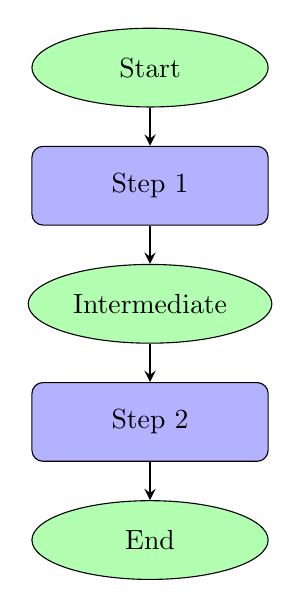
\begin{tikzpicture}[node distance=1.5cm]
\node (start) [object] {Start};
\node (step1) [process, below of=start] {Step 1};
\node (intermediate) [object, below of=step1] {Intermediate};
\node (step2) [process, below of=intermediate] {Step 2};
\node (end) [object, below of=step2]{End};

\draw [arrow] (start) -- (step1); 
\draw [arrow] (step1) -- (intermediate);
\draw [arrow] (intermediate) -- (step2); 
\draw [arrow] (step2) -- (end);
\end{tikzpicture}
\caption{A caption for the flowchart.}
\label{fig:comp}
\end{figure}

\section{Results}

This is the results section.

\begin{align}
	F &= ma \\
	\intertext{where:}
	F &= \text{net force applied on the body [N]} \nonumber \\
	m &= \text{total mass of the body [kg]} \nonumber \\
	a &= \text{net acceleration of the body [m s}^{-2}\text{]} \nonumber
\end{align}

\begin{figure}[htbp!]
	\begin{center}
		
\includegraphics[scale=0.7]{./images/catinhat}
	\end{center}
	\caption{A caption for the figure.}
	\label{fig:catinhat}
\end{figure}

\begin{table}[h]
	\centering
        \caption{A caption for the table.}
\begin{tabular}{lr}
	\hline
	\textbf{Properties} & \textbf{Value} \\
	\hline
    Mass [kg] & 2,324 \\
    Height [m] & 558 \\
    Volume [m$^3$] & 4,072 \\
    \hline
\end{tabular}
\label{tab:table1}
\end {table}

\section{Conclusions} \label{sec:conclusion}

This paper introduced the hybrid $S_N$-diffusion method for \gls{MSR} control rod neutronics
modeling. The hybrid $S_N$-diffusion method improves on the standard neutron diffusion method by
iteratively applying transport corrections generated from solving the $S_N$ neutron transport
method in subdomains containing highly neutron-absorbing control rods. The hybrid method uses the
\gls{SAAF} formulation of the $S_N$ equations, which are highly efficient and
scalable with HYPRE multigrid preconditioners \cite{hypre_hypre_2022} from PETSc.
Drift closure terms computed from the $S_N$ transport solution are passed as transport corrections
in modified forms of the neutron diffusion equations to correct flux errors in near control rods
where diffusion theory is not valid. This work also developed
an adaptive boundary coupling algorithm to couple the $S_N$ and neutron diffusion solvers. The
algorithm automatically truncates transport correction parameters near the boundaries of the
$S_N$ problem subdomain to discard inaccurate correction parameters and preserve smooth neutron
flux gradients across the interface. The $S_N$ and diffusion solvers are coupled through fixed
point iterations using the \gls{MOOSE} \texttt{MultiApp} and \texttt{Transfers} systems.

This paper presented 1-D and 2-D $k$-eigenvalue simulation results with the hybrid method on
models derived from the \gls{MSRE} reactor.
%The 1-D simulations involve six test cases with increasing
%geometric complexity modeled after the air-filled control rod thimbles, salt-graphite lattice
%structure, and vessel regions in the \gls{MSRE}.
Simulations with the OpenMC Monte Carlo neutron
transport code and the $S_8$ method in Moltres provided reference solutions for the hybrid and
neutron diffusion methods to be assessed against. Some discrepancies arose from the eight neutron
energy group structure as evidenced by differences in $k_\text{eff}$ and flux distributions between
OpenMC simulations on continuous energy (OpenMC-CE) and multigroup (OpenMC-MG) modes. Otherwise,
the multigroup $S_8$ method showed good agreement with OpenMC-MG. Although $k_\text{eff}$ estimates
from the hybrid method deviated from the $S_8$ method and OpenMC-MG by 100-400 pcm, the hybrid
method accurately reproduced control rod worth estimates within 0.5 \% of them (2-3 \% relative to
OpenMC-CE). In comparison, the neutron diffusion method fared significantly worse at 5.5 \%
relative to $S_8$ and OpenMC-MG, and 8 \% relative to OpenMC-CE. Our analyses showed little impact
on control rod worth estimates from varying the $S_N$-resolved subdomain size as long as the size
is kept constant between $k$-eigenvalue simulations used to calculate the rod worth. The hybrid
$S_N$-diffusion method exhibited a superlinear convergence rate with the number of fixed point
iterations, leading to the $k_\text{eff}$ error estimate falling below $10^{-7}$ after two
iterations.

The hybrid method maintained its accurate control rod modeling capability in 2-D simulations
involving incremental insertions of three control rods in the \gls{MSRE} model.
The hybrid method reported rod worth error magnitudes of less than 40 pcm relative to OpenMC-CE,
which were significant improvements over the neutron diffusion method error estimates ranging from
569 pcm to 1484 pcm. The hybrid method also showed significant improvements in the absolute mean
and maximum errors in fuel channel power distributions over the neutron diffusion method.

An extension to this work would be to resolve the discrepancies that persist in the hybrid method
$k_\text{eff}$ estimates of individual reactor states. Neutron leakage error at the external
boundaries is likely the most significant source of discrepancy and could be reduced through known
neutron leakage correction techniques such as group-wise or matrix albedo boundary conditions.
Further work is ongoing for the demonstration and performance characterization of the hybrid method
in $k$-eigenvalue and transient 3-D \gls{MSRE} simulations. Transient simulations under active
study include the zero-power rod drop and fractional-power reactivity insertion experiments
performed on the \gls{MSRE}. Future work would include asymmetrical power transients such as
partial channel flow blockage and potential in-core natural circulation flow following a loss of
pump power.

%The 3-D simulations in Chapter \ref{chap:msre} doubled as validation for the 3-D \gls{MSRE} model
%against reference \gls{MSRE} experimental data and the \gls{MSRE} numerical benchmark study
%\cite{fratoni_molten_2020} in
%the International Reactor Physics Experiment Evaluation Project (IRPhEP) handbook. OpenMC and
%hybrid method estimates of $k_\text{eff}$ of the \gls{MSRE} when the experiment first achieved criticality
%$k_\text{eff}$ estimates of the \gls{MSRE} at its initial critcality configuration from OpenMC, the
%hybrid method, and the neutron diffusion method in this work showed good agreement with the Serpent
%model from the \gls{MSRE} numerical benchmark. All numerical estimates exceeded the experimental
%value by 1-2 \% due to possible biases and uncertainties in the nuclear data library for graphite
%\cite{fratoni_molten_2020}. Temperature reactivity coefficient values from this work also showed
%good agreement with \gls{MSRE} data, within experimental uncertainty, with percentage discrepancies
%of about 3 \%. In the subsequent control rod worth study, OpenMC and the hybrid method showed nearly
%perfect overlap in the integral rod worth curve throughout the entire length of rod travel. Due to
%geometric approximations of the control rods in the numerical models, they overestimated the total
%rod worth relative to \gls{MSRE} data by approximately 4-5 \%. The hybrid method significantly
%outperforms the neutron diffusion method which overestimated the total worth by 21.1 \%.
%When comparing solution times, the hybrid method took approximately four times as long as the
%neutron diffusion method.
%The 3-D hybrid method simulations exhibited nearly linear scaling in strong scaling tests, which
%is promising for future projects involving larger reactor models. Some performance optimizations
%may be possible to reduce data transfer times between the $S_N$ and diffusion solvers which took
%up about 18 \% of the total solution time due to inter-processor communications.

%Lastly, Chapter \ref{chap:transient} demonstrated the hybrid method in a time-dependent simulation
%based on a \gls{MSRE} zero-power rod drop experiment \cite{prince_zero-power_1968}.
%The simulation required coupling the hybrid method solver to the pre-existing \gls{DNP} solver
%in Moltres through a nested iteration coupling setup.
%I set up the rod drop simulation through a
%$k$-eigenvalue simulation with the control rod at its initial height before using the simulation
%output as the initial condition for the time-dependent rod drop simulation. Moltres reproduced the
%expected prompt and delayed response in the integral neutron count data observed in \gls{MSRE}
%experimental data. Convergence issues midway through the simulation had a minor impact on the
%solution precision. Overall, this work successfully demonstrated a time-dependent
%reactivity-initiated simulation using the hybrid method.

%\subsection{Limitations and Future Work}

%The second \gls{VV} study verified the looped \gls{DNP} flow modeling capability in Moltres under
%steady-state and transient scenarios. In the original pump experiments, the control rod was driven
%by a ``flux servo controller'' that adjusts the rod position in response to flux changes to maintain
%criticality. Our study in this work approximated this action through $k$-eigenvalue solvers
%coupled to time-dependent \gls{DNP} flow solvers. Potential future work would be to implement a
%control system such as a PID (Proportional-Integral-Derivative) controller in combination with
%the newly-implemented hybrid method to create a more representative model of the pump experiments.
%This would enhance model validation and open up additional research directions which require a
%control system.
%
%This work implemented and verified the Spalart-Allmaras turbulence model in Moltres. The turbulence
%model \gls{VV} tests indicated significant mesh refinement requirements near the wall. Mesh
%refinement scales with the flow Reynolds number. With \gls{MSR} designs such as the \gls{MSFR}
%reaching Reynolds numbers on the order of $10^6$, future work in this area should focus on
%implementing wall functions. Wall functions eliminate the need for fine mesh near the wall by
%approximating the log-law velocity profile near the wall. Verification and demonstration of the
%turbulence model, beyond general \gls{VV} tests, in \gls{MSR} turbulent salt flow problems is also
%crucial for the continued development of Moltres as a \gls{MSR} simulation tool.

%The 3-D simulations in this work uncovered significant memory usage by the $S_N$ solver, even
%with the distributed mesh feature to spread mesh and variable data storage across the compute nodes.
%Each full-core simulation required at least 40 nodes with 512 GB memory each to run.
%This issue may be a stumbling block for using the hybrid method on smaller computing clusters that
%have less memory per processor. A custom preconditioner and solver routine in Moltres could help to
%reduce memory usage by referencing the same stored Jacobian C++ variable for neutron angular flux
%variables in the same neutron energy group and on the same \gls{FEM} quadrature point. Their
%Jacobian formulations are identical aside from the level-symmetric ordinate and weight. Another
%area for optimization in the hybrid method is reducing data transfer times between the $S_N$ and
%diffusion solvers. Due to mesh distribution, each 3-D simulation spent 18 \% of its solution time
%on data transfers between processors. This could be minimized through optimizations in the mesh
%distribution and the data transfer caching systems.
%
%Time-dependent simulations in this work uncovered two issues: rod cusping effects when a moving
%control rod does not align with the mesh interfaces, and slow solution convergence rates during
%control rod motion. While this work applied an empirical technique to correct for rod cusping
%effects, Moltres would benefit from a more robust technique for the long term. Slow solution
%convergence rates could be resolved by investigating better nested solver coupling structures to
%mitigate the effects of lagged solutions and applying solution relaxation schemes.
%
%Finally, future work could demonstrate the hybrid method to its fullest potential through the
%simulation of asymmetric reactivity-initiated transients. Asymmetry refers to significant changes
%in the neutron flux shape during a transient scenario. The core benefit of the hybrid method is
%the spatial resolution it provides to time-dependent simulations involving control rod movement.
%This objective could be met through modeling most other \gls{MSR} designs whose control and shim
%rods are not centrally located.

\section{Acknowledgments}
This is the acknowledgements section.
Include acknowledgements for relevant funding sources and contributors for
this work. Review the \href{https://drive.google.com/open?id=1VybV0oMPiqpInTwgO0ICq0EC4AL_fGj-zbXGJAhRiVU}{how-to-acknowledge}
document for the appropriate text, which changes frequently as grants and people
come and go.


\bibliography{bibliography}

% Prof. Huff discourages appendices in journal articles.
% But, if you must, include one like so:
%\pagebreak
%
\appendix
\section{}


\end{document}
